\documentclass[11pt]{article}

% Use the following to compile
% mkdir tmp
% pdflatex -aux-directory=tmp -output-directory=tmp --shell-escape notes.tex

% Use the following to compile
% mkdir tmp
% pdflatex -aux-directory=tmp -output-directory=tmp --shell-escape notes.tex

% Package use definitions
\usepackage[top=2.5cm, bottom=2.5cm]{geometry}
\usepackage{fancyhdr}
\usepackage{graphicx}
\usepackage{comment}
\usepackage[outputdir=/tmp]{minted}
\usepackage[dvipsnames]{xcolor}
\usepackage{listings}
\usepackage[hidelinks]{hyperref}
\usepackage{amsmath}
\usepackage{amsfonts}
\usepackage{amssymb}
\usepackage{tcolorbox}
\usepackage{multicol}
\usepackage{titlesec}
\usepackage{bbm}
\usepackage{verbatim}
\usepackage{varwidth}

\titleformat{\section}
            {\large\bfseries}{\thesection.}{2mm}{}
\titleformat{\subsection}
            {\large\bfseries}{\thesubsection.}{2mm}{}
\titleformat{\subsubsection}
            {\large\bfseries}{\thesubsubsection.}{2mm}{}

% Column Separation
\setlength{\columnsep}{1cm}

% Settings minted option for the entire document
\definecolor{LightGray}{gray}{0.9}
\setminted{frame=lines,framesep=2mm,bgcolor=LightGray,linenos,
  fontsize=\footnotesize, baselinestretch=1.2}

% Start of document
\begin{document}

% Title page and table of contents setup
\begin{titlepage}
    \begin{center}
    \Huge \textbf{A Simulated Annealing solution to the Tetravex game}\\
    \vfill
    \end{center}
    \textbf{Abstract} This report shows my solution to the Tetravex game. As
    directed, the program makes use of the Simulated Annealing algorithm to find
    its solution. This report shall first present the Simulated Annealing
    algorithm, then it shall present some notes on the implementation process of
    this algorithm into the final program. Then the following section shall
    present some of the optimizations that were considered and implemented to
    improve the execution time. Then finally the report shall present the final
    results, some possible improvements, and shall end with a conclusion.
    \vfill
     \tableofcontents
  \begin{center}
    \vfill
    \normalsize \textbf{Jose A. Henriquez Roa}\\
    \vspace*{2\baselineskip} \today \rhead{\today}
  \end{center}
\end{titlepage}

\newgeometry{includeheadfoot, left=1.5cm, right=1.5cm, top=1cm, bottom=1cm,
  headsep=10mm, footskip=15mm}
% Header and footer setup
\pagestyle{fancy}
\rhead{}
\lhead{A Simulated Annealing solution to the Tetravex game}
\renewcommand{\headrulewidth}{1pt}
\renewcommand{\footrulewidth}{1pt}

% Document Body:
\begin{multicols*}{2}
  \section{Introduction}
  \subsection{The Tetravex game}
  The tetravex game is an edge-matching puzzle inspired by some of the work
  presented by Knuth began in his book series The Art of Computer Programming
  [1]. The game itself was invented by Scott Ferguson for the Windows
  Entertainment Pack which was released in 1991. Since then an open source
  version has been made available in the GNOME Games collection under the name
  \texttt{gnome-tetravex}. This same executable was used to generate some
  solvable board examples that were used to test the presented program
  implementation.\\\\ The game itself is made up of a square grid board and a
  set of tiles. In the gnome-tetravex version of the game, the board size ranges
  from a 2x2 to a 6x6 grid. The titles themselves are made up of four numbers
  (usually 0 to 9) at each of side, and the total number of tiles matches the
  grid size. The goal of the game is to place all of the tiles in the grid as
  such that each side of each tile matches with the number of their four
  adjacent neighbors. A solved tetravex board example is given in the following
  figure
  \ref{fig:solved-board-example}.
\begin{figure}[H]
  \centering
  \fontsize{11pt}{11pt}\selectfont
  \begin{varwidth}{\linewidth}
    \verbatiminput{txt/board3.txt}
  \end{varwidth}
  \caption{3x3 Solved board example}
  \label{fig:solved-board-example}
\end{figure}
\subsection{Program compilation \& execution}
Before moving on to the following section presenting the algorithm and the
implementation we shall first give some few notes on the compilation and
execution of the program.\\\\ There is a total of 3 files in the presented
program, two source files and one header file. These are respectively
\texttt{main.cc}, \texttt{tetravex.cc} and \texttt{tetravex.hh}. All of the
logic related to loading input files, solving and writing out the output file
is contained in the tetravex.cc source file.\\\\ As instructed the entire program
can be executed by simply executing the following command the root
directory:\\\\ \texttt{\$ g++ -std=c++17 *.cc}\\\\
This will output an \texttt{a.out} binary file that should be executed through
the following command:\\\\ \texttt{\$ ./a.out in.txt out.txt}\\\\
Where \texttt{in.txt} should be in the following format:
\begin{figure}[H]
  \centering
  \fontsize{11pt}{11pt}\selectfont
  %% \hfill
  \begin{varwidth}{\linewidth}
    \verbatiminput{txt/board2-input.txt}
  \end{varwidth}
  \qquad\quad
  \begin{varwidth}{\linewidth}
    \verbatiminput{txt/board2.txt}
  \end{varwidth}
  %% \hfill
  \caption{2x2 Board input file contents example (left) and associated board
    representation (right)}
  \label{fig:input-file-example}
\end{figure}
\noindent Where each line defines a tile in the format
\texttt{<north><west><east><south>} in their respective initial position in the
grid. The \texttt{@} symbol specifies that the tile is fixed in its initial
position and shall not be moved while attempting to solve the board. This
implementation handles input files without any fixed tile marker.\\\\ The output
file shall present the solved board in the same format as the input file, but
without the use of any fixed tile markers.
\section{Simulated Annealing}
This section shall present the algorithm and the main concepts that were used to
solve the Tetravex problem in the presented program implementation. The
algorithm that was used to solve the problem is the simulated annealing
algorithm introduced in the 1983 paper ``Optimization by Simulated Annealing'' [3],
this one is based on the Metropolis Hastings algorithm which itself was
presented in the 1953 paper ``Equation of State Calculations by Fast Computing
Machines'' [2].\\\\ This section shall first present some concepts of the Finite
Markov Decision Process which are required before moving on to the following
section on the Simulated Annealing algorithm.
\begin{figure*}[t]
  \centering
  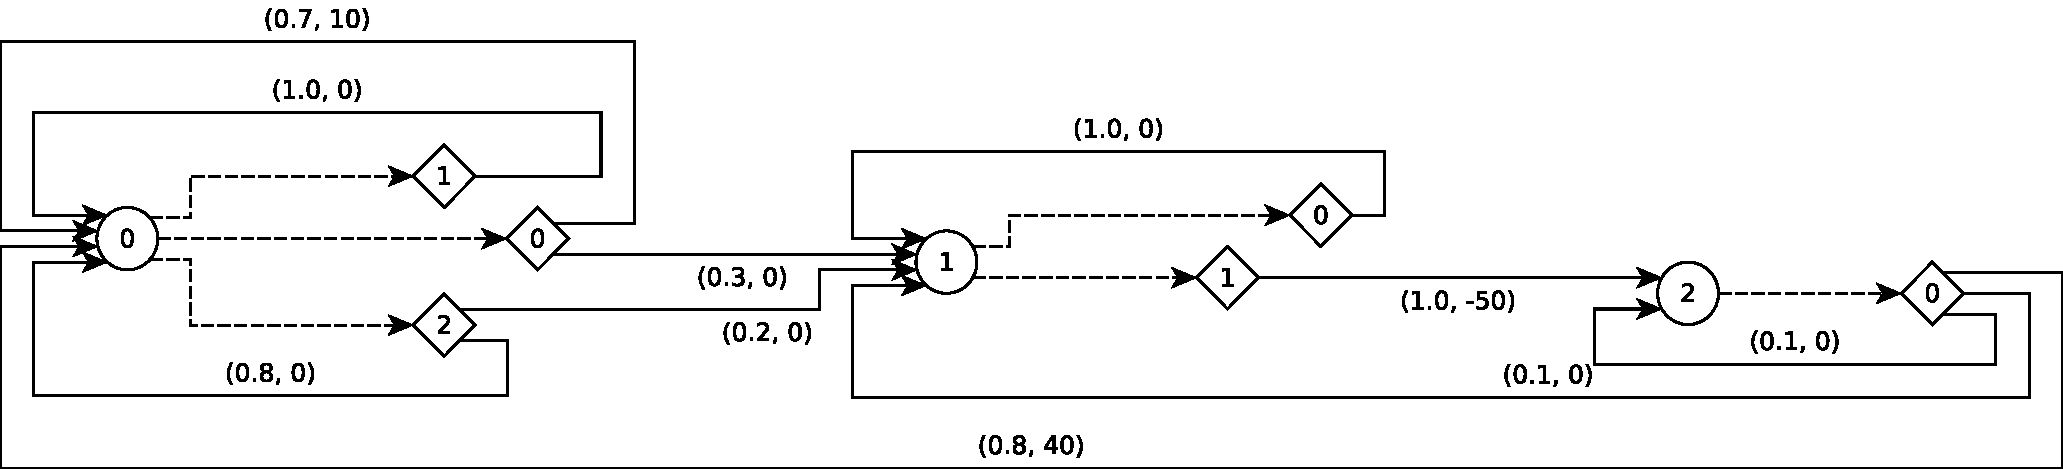
\includegraphics[width=\linewidth]{image/mdp.pdf}
  \caption{Markov Decision Process diagram. The circles represent the states
    and the diamonds the actions. In this diagram there is only one possible
    reward when passing to a state $s^\prime$ after choosing an action $a$,
    this is not always the case.}
  \label{fig:mdp}
\end{figure*}
\subsection{Finite Makov Decision Process}
\noindent An example of a Makov Decision Process (MDP) is given in figure
\ref{fig:mdp}. To present what an MDP is we shall use the agent-environment
analogy. An MDP is a stochastic model that defines all of the possible
interaction between an agent in a specific environment. At each state (circle)
the agent is presented a set of actions (diamonds). When an action $a$ is chosen
by an agent in a given state $s$ then the environment responds by changing the
state to a new one $s^\prime$ and giving a reward $r$ depending on a predefined
(sometimes unknown) transition probability.\\\\ Do note however that the
following algorithms use a special type of MDPs called Markov Chains. Which are
essentially are MDPs with only one action and for which the rewards are
neglected (e.i set to zero). The choice to present MDPs instead of directly
presenting Markov Chains was to introduce the concept of \textit{reward} which
is used to simplify the presentation of the following algorithms.
\subsection{Simulated Annealing algorithm}
The Simulated Annealing algorithm is based on the Metropolis–Hastings algorithm,
The later is a method of generating a Markov Chain from a probability
distribution. And the former is a variant of this one used for optimization.\\\\
The simulated annealing algorithm is rather straightforward at each iteration the
algorithm considers transitioning to a new state $s^\prime$ from the current
state $s$. The probability of actually transitioning to the new state depends on
two components. First a loss function, which defines a relative ordering in
between the possible states, more attractive states will have a smaller
loss. And a temperature, which regulates how likely the algorithm is to
transition to less attractive states, with a higher temperature meaning that
less attractive states are more likely to be considered.\\\\
There are many variants for the acceptance probability, however, the one that
was considered for the presented implementation is:
\begin{equation}
  p = e^\frac{-L(s^\prime) - L(s)}{T}
\end{equation}
Where $L$ is the loss function, $T$ is the temperature, $s^\prime$ is the new
state being considered and $s$ is the current one.\\\\ The algorithm attempts to
converge to an optimal solution by decreasing the temperature at each iteration,
this has the effect of first allowing the algorithm to sufficiently explore the
state space when the temperature is high and constraining it to choose the most
attractive states when the temperature is low.\\\\ In regards to the loss
function we note it's similarities with the rewards in MDPs. Drawing a parallel
to some Reinforcement Learning (RL) concepts, the loss function defines the same
concept as the optimal state value function $v_*(s)$ is RL, this is is defined
as the expected \textit{return} when starting in state $s$ and choosing future
actions according to the optimal policy. We can then interpret the problem the
Simulated Annealing algorithm is trying to solve as trying to find the optimal
state given the state value function.\\\\ Going back to the original Tetravex
problem. In the presented implementation the state space defined by all of the
possible grid configurations. And the loss function is defined such as it
decreases by 1 for every matching side of each tile. Each matching pair is
counted exactly only once and not twice, or once for each tile.\\\\ The initial
loss is set to 0 which makes the optimal loss equal to $l^* = -2(n^2-n)$, where
$n$ is the side of the grid being solved.
\begin{figure*}[t]
  \centering
  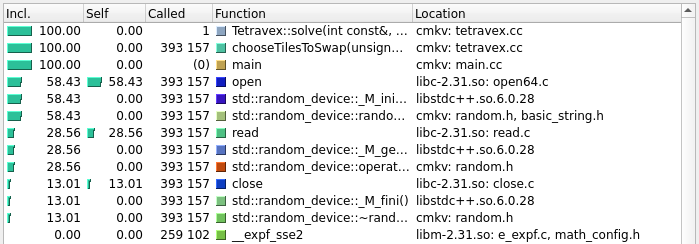
\includegraphics[scale=0.5]{image/error.png}
  \caption{Code profile}
  \label{fig:callgrind}
\end{figure*}
\section{Optimizations}
\subsection{Simulated Annealing optimization}
The algorithm was optimized in two aspects. First, by searching for a good
initial Temperature $T_0$. And second, by making modification to the annealing
schedule (process used to decrease the temperature at each iteration).\\\\ The
search for $T_0$ parameter was done manually by tuning this one all through the
development by testing it against multiple input board of different
sizes.\\\\ For the annealing schedule, this one required more research to be
performed. Initially the temperature was decreased linearly and was simply reset
when the algorithm did not manage to find the solution before the temperature
reached 0. However, this was much improved upon, currently the algorithm is set
to decrease the temperature as such that 0 is reached at a given predefined max
time-step $t_{max}$. With this new method there is no longer need to completely
reset the board (by resetting the temperature). Now, when the algorithm does not
manage to find a solution in time and reaches $t_{max}$, $t_{max}$ will simply
be increased by a predefined value (which will also increase the temperature)
and allow the algorithm to the out of any sort of local minima, all without
having to restart from 0.
\subsection{General program optimizations}
Some additional optimization were performed on the source code side of things.
During the implementation the algorithm featured a surprisingly high execution
time, even for board of small size. Profiling the code resulted in the
\texttt{callgrind} results shown in figure \ref{fig:callgrind}. In this ones we
see that by far most of the execution time was spent on the member function of
the Tetravex class \texttt{chooseTilesToSwap()}, which itself was part of the
smallest simpler function in the main loop in \texttt{solve()}. Further
inspection showed that there was a unusually high amount time being spent on
kernel calls. This was later on found out to be due to the usage of the
\texttt{std::default\_random\_engine} class, which was used to generate the
random number used to randomly select movable tiles. Fixing this issue allowed
to decrease the execution time by a factor of over 100.
\section{Results}
\subsection{Execution time sampling}
The two Bash and Python presented in figures \ref{fig:time} and \ref{fig:stat}
were used for both tuning the parameters of the Simulated Annealing algorithm
as well as for computing the final execution time analysis presented in the
following section.\\\\
\begin{figure}[H]
  \centering
  \begin{minipage}{0.5\textwidth}
  \begin{minted}{bash}
 g++ -std=c++17 *cc
  
 grid_size=6

 echo "exec_time" > $grid_size.csv
 for i in $(seq 100); do
   ./a.out in-$grid_size.txt out-$grid_size.txt \
   >> $grid_size.csv
 done
  
 python3 stat.py $grid_size.csv
  \end{minted}
  \end{minipage}
  \caption{time.sh: Bash script for collecting execution times}
  \label{fig:time}
\end{figure}
\begin{figure}[H]
  \centering
  \begin{minipage}{0.5\textwidth}
    \begin{minted}{python}
 import sys, pandas

 print(pandas.read_csv(sys.argv[1]).describe())
    \end{minted}
  \end{minipage}
  \caption{stat.py: Python for getting execution time statistics}
  \label{fig:stat}
\end{figure}
\noindent The \texttt{time.sh} script was used to generate a CSV file containing the
execution times of the \texttt{solve()} function. And the \texttt{stat.sh} was
used to generate some useful statistics from the previously sampled execution
times.
\subsection{Execution time analysis}
The following table show multiple statistics related to the sampled execution
times of the presented program on the multiple board sizes ranging from 2x2 to
6x6 in seconds. For these tests only input boards without fixed tiles were given
to the program.
\begin{figure}[H]
  \centering
  \begin{tabular}{|| c c c c c c ||}
    \hline
    Stat. & 2x2 & 3x3 & 4x4 & 5x5 & 6x6\\ [0.5ex]
    \hline\hline
    mean & 6.4e-5 & 0.02 & 0.27 & 0.97 & 10.92\\
    std  & 2.7e-5 & 0.02 & 1.34 & 1.54 & 8.96\\
    min  & 1.6e-5 & 2.1e-3 & 7.1e-3 & 0.02 & 0.28\\
    25\% & 4.7e-5 & 4.5e-3 & 9.2e-3 & 0.10 & 4.30\\
    50\% & 5.9e-5 & 0.01 & 0.01 & 0.19 & 8.58\\
    75\% & 7.7e-5 & 0.03 & 0.03 & 1.22 & 15.01\\
    max  & 1.4e-5 & 0.12 & 10.56 & 8.17 & 46.68\\
    \hline
  \end{tabular}
  \caption{Execution times statistics averaged accross 100 samples in seconds}
  \label{fig:exec-stat}
\end{figure}
\section{Improvements}
The following is a list of possible improvements:
\begin{enumerate}
\item Consider other annealing algorithms aside from the Simulated Annealing
  one. Or implement other methods for solving the problem all together, for this
  Reinforcement Learning could be considered.
\item Do some additional parameter tuning.
\item Implement a multi-threaded version that for each thread shuffles the board
  and launches a \texttt{solve()} instance. This method would decrease the
  execution time variance.
\end{enumerate}
\section{Conclusion}
As directed we made use of a Metropolis–Hastings variant, in this case Simulated
Annealing, to implement a Tetravex solver. Through the implementation process,
extensive research was made on the algorithm and all of its related concepts.
Particularly after having implemented a working version, while trying to further
optimize the current implementation.
\end{multicols*}
\end{document}
